% include the figures path relative to the master file
\graphicspath{ {./content/intro/figures/} }

\section{Introduction}
\label{sec:intro}  % \label{} allows reference to this section

  \added[id=old]{
    Eye diseases such as \gls{dr} and \gls{dme} are the most common causes of
    irreversible vision loss in individuals with diabetes.  Just in United States
    alone, health care and associated costs related to eye diseases are estimated
    at almost \SI{500}[\$]{M}~\cite{Sharma2005}.  Moreover, the prevalent cases of
    \gls{dr} are expected to grow exponentially affecting over \SI{300}{M} people
    worldwide by 2025~\cite{Wild2004}.  Given this scenario, early detection and
    treatment of \gls{dr} and \gls{dme} play a major role to prevent adverse
    effects such as blindness.  \gls{dme} is characterized as an increase in
    retinal thickness within 1 disk diameter of the fovea center with or without
    hard exudates and sometimes associated with cysts~\cite{ETDRSG1985}.  Fundus
    images which have proven to be very useful in revealing most of the eye
    pathologies~\cite{Mookiah20132136,Trucco2013} are not as good as \gls{oct}
    images which provide information about cross-sectional retinal
    morphology~\cite{Wang2015}.
  }

  %Indeed, the new generation of \gls{oct} imaging, namely \gls{sdoct} offers high resolution and fast image acquisition, producing from $27,000$ to $40,000$ A-scans/second with an axial resolution ranging from \SIrange{3.5}{6}{\micro \metre}~\cite{Chen2005}.
\begin{figure}
  \begin{center}
    \hspace*{\fill}
      \subfigure[Normal]{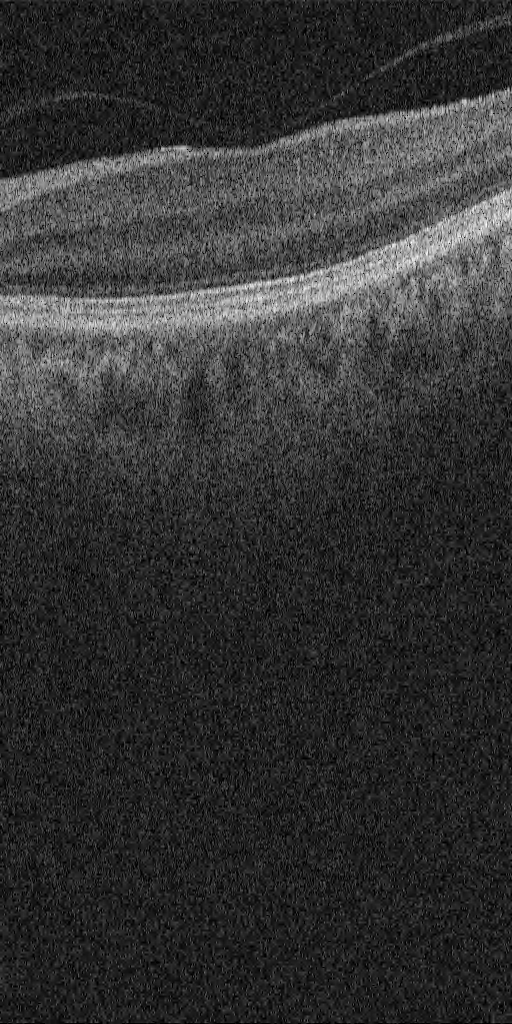
\includegraphics[scale=0.15]{normal_case}}\hfill
      \subfigure[\gls{dme}-cyst]{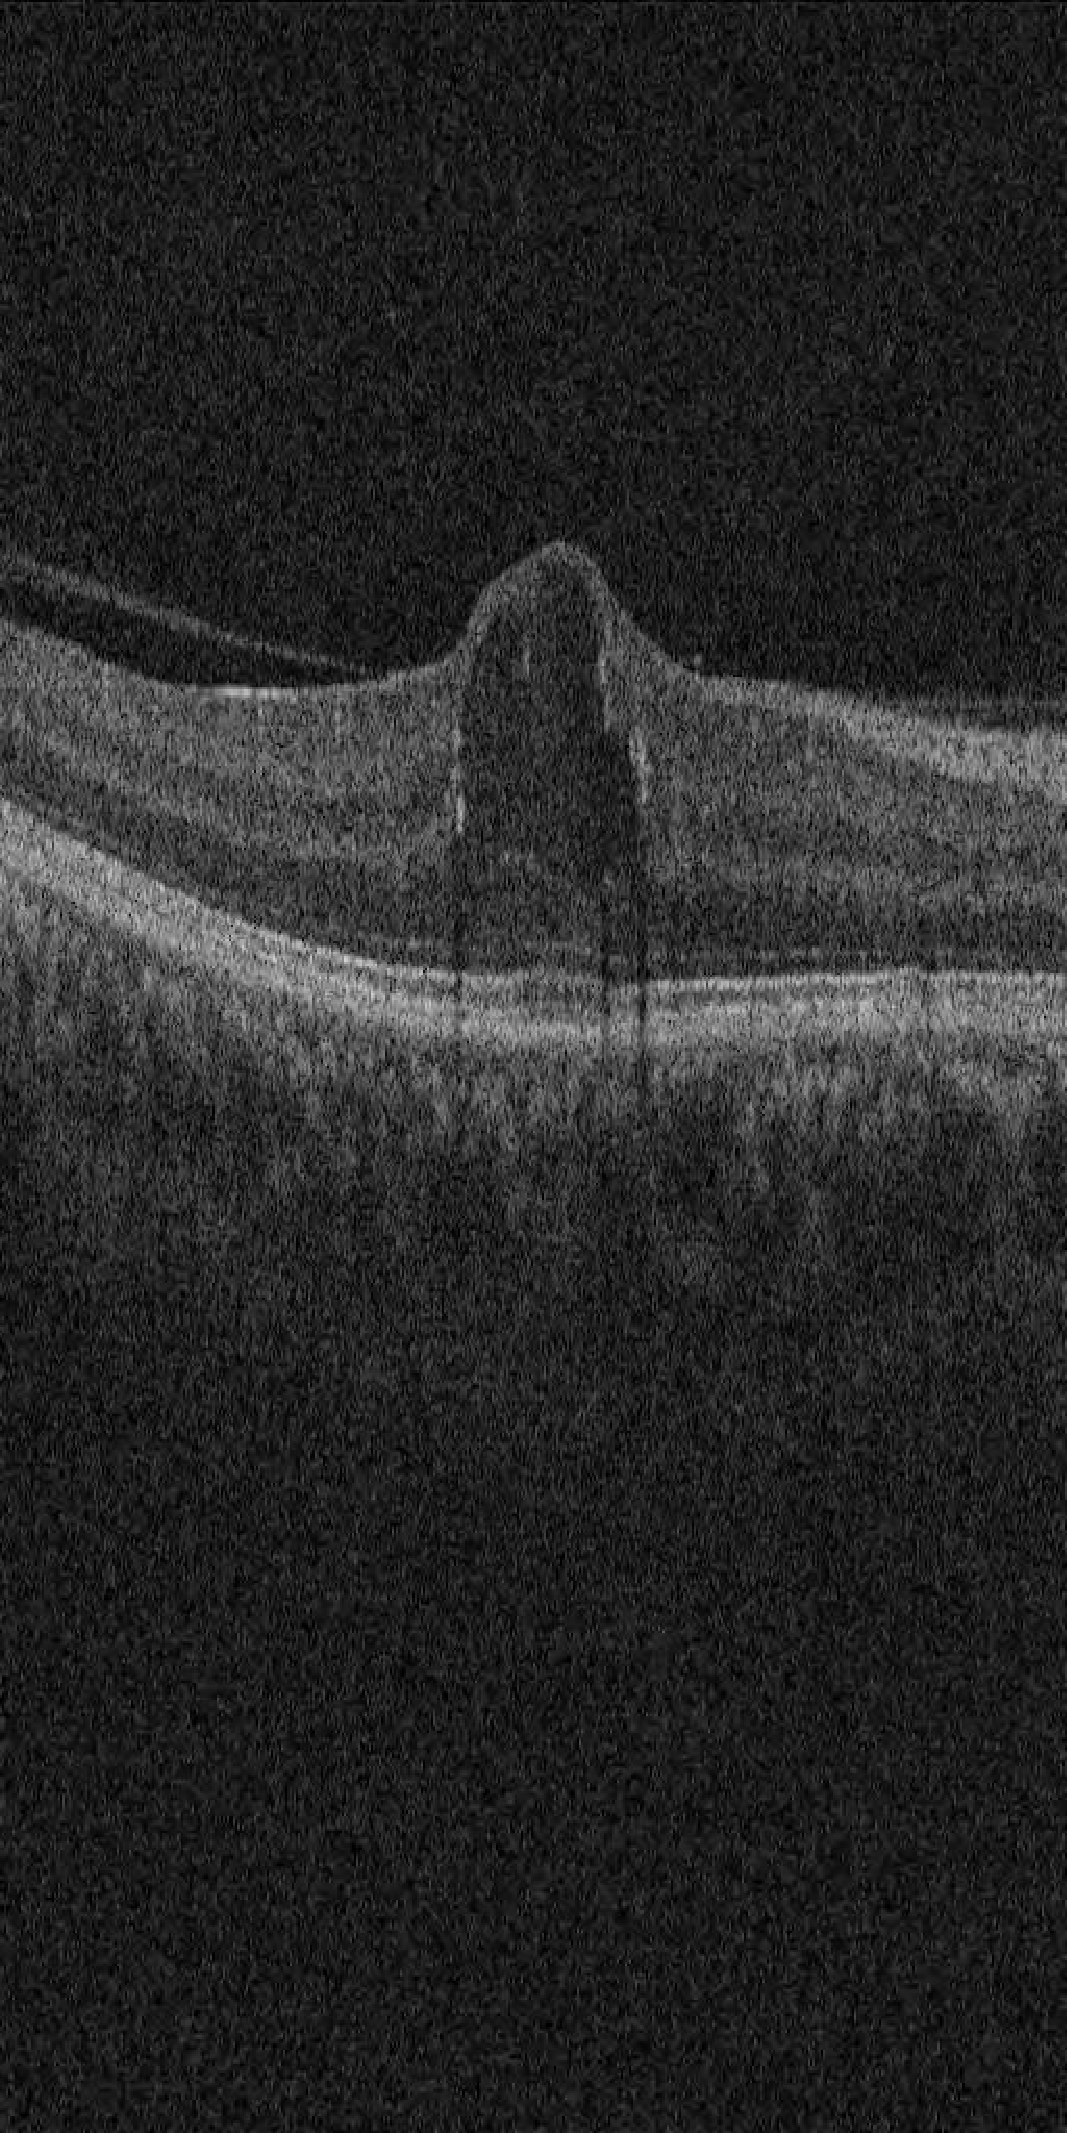
\includegraphics[scale=0.15]{dme_cyst}}\hfill
      \subfigure[\gls{dme}-exudate]{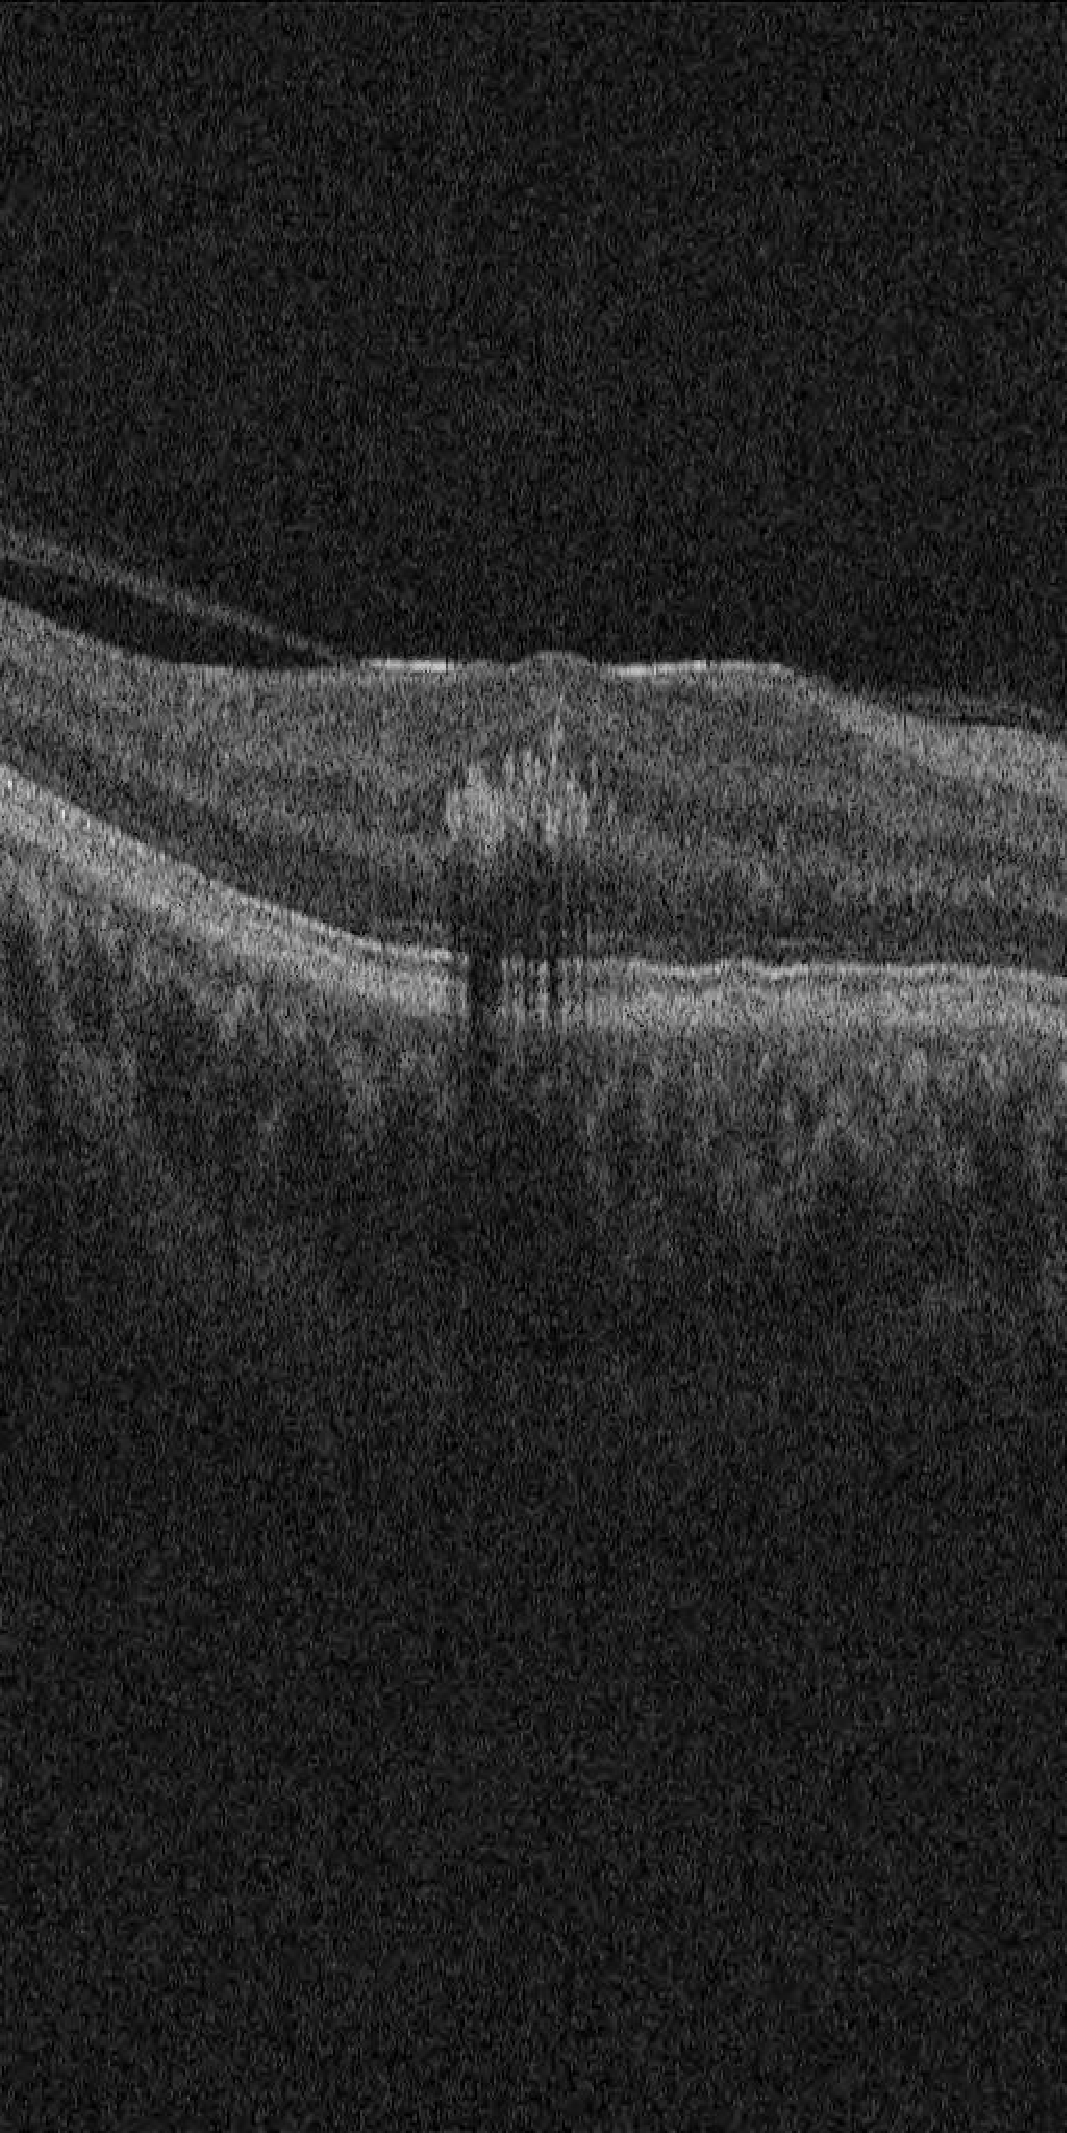
\includegraphics[scale=0.15]{dme_exudate}}
      \hspace*{\fill}
  \end{center}
  \caption{ Example of \gls{sdoct} images for normal (a) and \gls{dme} patients (b)-(c) with cyst and exudate, respectively.}
  \label{fig:dme-normal}
\end{figure}

  \added[id=old]{
    Many of the previous works on \gls{oct} image analysis have focused on the problem of retinal layers segmentation, which is a necessary step for retinal thickness measurements~\cite{Chiu2010,Kafieh2013}.
    However, few have addressed the specific problem of \gls{dme} and its associated features detection from \gls{oct} images.
    Figure\,\ref{fig:dme-normal} shows one normal B-scan and two abnormal B-scans.
  }


  Evaluation of the volumetric scan is time consuming, expensive
  and some pathology signs are easy to miss~\cite{Venhuizen2015}

  \deleted[id=sik]{
  $\cdot$ coexistence of multiple pathologies~\cite{Liu2011}
  $\cdot$ OCT image acquisition has drift~\cite{Liu2011}
  $\cdot$ variability in shape, size and magnitude within the same pathology~\cite{Liu2011}
  $\cdot$ retina reflectivity (schuman 2014)~\cite{Liu2011}
  $\cdot$ inconsistent image quality (barnum 2008)~\cite{Liu2011}
  }

  \deleted[id=sik]{
    This article is structured as follows: Background(Sect.\,\ref{sec:survey}) offers a general idea of the methods reviwed.
    Materials and methods discusses data and mapping of the methodologies to our framework.
    Results offers (Sect.\,\ref{sec:results}) (a) individual results of each methodology, as well as our strategy followed to validate that our implementation complies with the results reported by the original work
    (b) comparative results of the best methodlogy configurations to drive our discussion.
    Discussion(Sect.\,\ref{sec:discussion}). Conclusion and Further work(Sect.\,\ref{sec:conclusion}).
  }

% Some stuff that emac's colegues use
%%% Local Variables:
%%% mode: late
%%% TeX-master: "../../main.tex"
%%% End: \section{introduction}

